\documentclass[a4paper,12pt]{article} 

%%% Работа с русским языком
\usepackage{cmap}					% поиск в PDF
\usepackage{mathtext} 				% русские буквы в фомулах
\usepackage[T2A]{fontenc}			% кодировка
\usepackage[utf8]{inputenc}			% кодировка исходного текста
\usepackage[english,russian]{babel}	% локализация и переносы

%%% Дополнительная работа с математикой
\usepackage{amsmath,amsfonts,amssymb,amsthm,mathtools, gensymb} % AMS
\usepackage{icomma} % "Умная" запятая: $0,2$    ф--- число, $0, 2$ --- перечисление

%%Таблица
\usepackage[table,xcdraw]{xcolor}
\usepackage{caption}
\usepackage{floatrow}
\floatsetup[table]{capposition=top}
\floatsetup[wrapfigure]{capposition=bottom}

%Отступы и поля 
\textwidth=18cm
\oddsidemargin=-1cm
\topmargin=-2cm
\textheight=25cm


%% Номера формул
\mathtoolsset{showonlyrefs=true} % Показывать номера только у тех формул, на которые есть \eqref{} в тексте.

%% Шрифты
\usepackage{euscript}	 % Шрифт Евклид
\usepackage{mathrsfs} % Красивый матшрифт

%% Свои команды
\DeclareMathOperator{\sgn}{\mathop{sgn}}

%% Перенос знаков в формулах (по Львовскому)
\newcommand*{\hm}[1]{#1\nobreak\discretionary{}
{\hbox{$\mathsurround=0pt #1$}}{}}

%% Стиль страницы
\usepackage{fancyhdr}

%% Для рисунков
\usepackage{graphicx}
\usepackage[export]{adjustbox}
\usepackage{float}
\usepackage{ragged2e}
\usepackage{wrapfig}

\pagestyle{fancy}
\begin{document}
\begin{titlepage}
\begin{center}
%\vspace*{1cm}
\large{\small ФЕДЕРАЛЬНОЕ ГОСУДАРСТВЕННОЕ АВТОНОМНОЕ ОБРАЗОВАТЕЛЬНОЕ\\ УЧРЕЖДЕНИЕ ВЫСШЕГО ОБРАЗОВАНИЯ \\ МОСКОВСКИЙ ФИЗИКО-ТЕХНИЧЕСКИЙ ИНСТИТУТ\\ (НАЦИОНАЛЬНЫЙ ИССЛЕДОВАТЕЛЬСКИЙ УНИВЕРСИТЕТ)\\ ФАКУЛЬТЕТ АЭРОКОСМИЧЕСКИХ ТЕХНОЛОГИЙ}
\vfill
\line(1,0){490}\\[1mm]
\huge{Лабораторная работа 3.4.5}\\
\huge\textbf{Петля гистерезиса (динамический метод)}\\
\line(1,0){490}\\[1mm]
\vfill
\begin{flushright}
\normalsize{Рогозин Владимир}\\
\normalsize{\textbf{Группа Б03-106}}\\
\end{flushright}
\end{center}
\end{titlepage}
\fancyhead[L] {Работа 3.4.5}


\textbf{Цель работы}: 
изучение петель гистерезиса различных ферромагнитных материалов в переменных полях.

\textbf{Оборудование}:
автотрансформатор, понижающий трансформатор, интегрирующая цепочка, амперметр, вольтметр, электронный осциллограф, делитель напряжения, тороидальные образцы с двумя обмотками.

\textbf{Теоретические сведения}:
Помимо диа- и парамагнетиков, которые слабо реагируют на внешнее магнитное поле, в природе существуют вещества, способные сильно намагничиваться даже в небольших полях. Такие вещества относят к классу \textit{ферромагнетиков}. Зависимость намагниченности $\mathbf{M}$ от напряжённости магнитного поля $\mathbf{H}$ у всех ферромагнетиков оказывается нелинейной: магнитная восприимчивость $\mathbf{\chi}$ не является константой и зависит от $\mathbf{H}$. Кроме того, анизотропия кристаллической решётки приводит к тому, что $\mathbf{\chi}$ может иметь тензорный характер.

Как и в случае парамагнетиков, атомы ферромагнетика обладают собственным магнитным моментом. Однако даже в отсутствие внешнего магнитного поля атомы ферромагнетика способны образовывать упорядоченные структуры (\textit{домены}), в которых все магнитные моменты ориентированы практически в одном направлении. Таким образом, каждый отдельный атом испытывает влияние не только внешнего поля, но и поля, созданного коллективом его соседей.

\textbf{Модель среднего поля.} 
В качестве простейшей эмпирической модели, описывающей такую ситуацию, можно рассмотреть следующую модель: предположим, что намагниченность элемента среды пропорциональна некоторому эффективному полю $\mathbf{H}_{эфф}$, складывающемуся из поля $\mathbf{H}$ в данной точке, созданного сторонними токами, и среднего «коллективного» поля, пропорционального величине намагниченности $\mathbf{M}$:
\[\mathbf{M} = \chi_{пар} \mathbf{H}_{эфф}, \quad \mathbf{H}_{эфф} = \mathbf{H} + \beta \mathbf{M},\]
где $\chi_{пар}$ -- парамагнитная восприимчивость отдельного атома, $\beta$ -- некоторая безразмерная константа, определяемая из опыта. 

Модель среднего поля позволяет уточнить закон Кюри. Определяя
магнитную восприимчивость по-прежнему как $\chi = M / H$,  найдём:
\[\chi = \frac{1}{\chi_{пар}^{-1} - \beta} \propto \frac{1}{T - \Theta},\]
где параметр $\Theta$ имеет размерность температуры.

Это соотношение называют \textit{законом Кюри-Вейсса}. Он предсказывает существование особой точки -- температурной \textit{точкой Кюри} $\Theta_к$ в которой имеет место фазовый переход 2-го рода между парамагнитным (при $T > \Theta_к$) и ферромагнитным (при $T < \Theta_к$) состояниями среды. Закон Кюри-Вейсса удовлетворительно выполняется вдали от $\Theta_к$, однако нарушается при приближении к точке перехода, где модель среднего поля становится слишком груба.

\textbf{Образование доменов.} 
Магнитное (диполь-дипольное) взаимодействие между атомами не может привести к упорядочению системы, так как его энергия слишком мала по сравнению с энергией теплового движения молекул уже при температурах порядка $T \sim 1$ К. Единственное взаимодействие, которое способно выстроить в ряд магнитные моменты электронов в атомах при температурах порядка комнатной, -- это электростатическое взаимодействие. Как следует из квантовой механики, если магнитные моменты (или спины) электронов соседних атомов сонаправлены, их электростатическое отталкивание становится меньше. Таким образом, магнитным моментам атомов энергетически выгодно ориентироваться в одном направлении. Такое явление получило название \textit{обменного взаимодействия.} 

С другой стороны, магнитное дипольдипольное взаимодействие между доменами препятствует выстраиванию всех магнитных моментов среды в одном направлении. Действительно, энергия такого взаимодействия будет минимальной при антипараллельном расположении магнитных моментов соседних элементов среды. Поэтому при определённом поперечном размере домена оказывается энергетически выгодно иметь соседний домен с противоположно ориентированным моментом. Наложение внешнего поля заставляет домены ориентироваться по нему, что приводит к резкому увеличению намагниченности образца, а при достаточно большом поле достигается состояние \textit{насыщения}, когда все домены ориентируются по полю. 

\textbf{Ферромагнитный гистерезис.} 
Если состояние некоторой системы зависит не только от мгновенных значений внешних параметров, но от истории их изменений, говорят, что в системе имеет место \textit{гистерезис}.

Именно такими свойствами обладает магнитный момент ферромагнитного образца как функция напряжённости поля $M(H)$. В частности, система может оказаться намагниченной, даже когда внешнее поле выключено -- этим объясняется существование постоянных магнитов.
\begin{figure}[H]\label{fig: Гистерезис картинка}
    \centering
    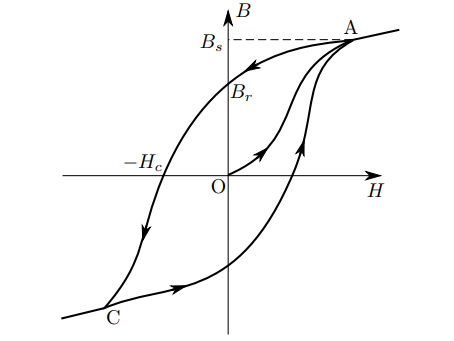
\includegraphics[width = 0.7\textwidth]{Гистерезис картинка.png}
    \caption{Начальная кривая намагничивания (OA) и предельная петля гистерезиса}
\end{figure}
Наклон кривой намагничивания характеризуется \textit{дифференциальной магнитной проницаемостью}
\[\mu_{диф} = \frac{1}{\mu_0} \frac{dB}{dH} .\]
С ростом $H$ величина $\mu_{диф}$ сначала растёт, затем начинает резко падать,
 приближаясь к единице при насыщении.

Доведём систему до некоторой точки $A$, лежащей в области насыщения (здесь $B_s$-- индукция насыщения), и начнём уменьшать напряжённость $H$. Поскольку между доменами есть трение, обратный путь пойдёт не по начальной кривой, а выше неё.
При выключения внешних полей, то есть при достижении $H = 0$, в образце сохраняется некоторое собственное намагничивание. Соответствующее значение индукции $B_r$ называют \textit{остаточной индукцией}. Значение $B = 0$ достигается лишь при некотором отрицательном значении $H = - H_c$. Величина $H_c$ называется \textit{коэрцитивным полем}. В точке $C$ наступает насыщение для намагничивания в противоположную сторону.

Если теперь попробовать вернуться в точку $A$, вновь наращивая поле, получим некоторый замкнутый цикл (предельную \textit{петлю гистерезиса}). Если в точке $A$ насыщение не достигается, то аналогичным образом получится цикл меньшей площади. 

Отметим, что площадь петли гистерезиса ферромагнетика на плоскости $H-B$ есть энергия, необратимо выделяющаяся в виде тепла в единице объёма вещества за один цикл:
\[\Delta \omega = - \oint H dB.\]


\textbf{Экспериментальная установка}:
В данной работе кривые гистерезиса ферромагнитных материалов изучаются в поле частоты $\nu_0 = 50$ Гц с помощью электронного осциллографа.

Магнитную индукцию $B$ удобно определять с помощью ЭДС, возникающей при изменении магнитного потока $\Phi$ в катушке, намотанной на образец. Пусть катушка c $N$ витками плотно охватывает образец сечением $S$, и индукция $B$ в образце
однородна. Из закона электромагнитной индукции получаем
\[|B| = \frac{1}{S N} \int \varepsilon dt.\]
Таким образом, для определения $B$ нужно проинтегрировать сигнал, наведённый меняющимся магнитным полем в измерительной катушке, намотанной на образец.

Для интегрирования в работе используется интегрирующая $RC$-цепочка. «Входное» напряжение от источника $U_{вх}(t)$ подаётся на последовательно соединённые резистор $R_{и}$ и конденсатор $C_{и}$. «Выходное» напряжение $U_{вых}(t)$ снимается с конденсатора. Предположим, что 1) сопротивление источника мало по сравнению с $R_{и}$, 2) выходное сопротивление (сопротивление на входе осциллографа), напротив, велико: $R_{вых} \gg R_{и}$ и 3) сопротивление $R_{и}$ достаточно велико, так что почти всё падение напряжения приходится на него, а $U_{вых} \ll U_{вх}$. В таком случае ток цепи равен $I$ = $U_{вх} - U_{вых} / R_{и} \approx U_{вх} / R_{и}$, и входное и выходное сопротивление связаны соотношением
\[U_{вых} = \frac{q}{C_и} = \frac{1}{C_и} \int_0^t I dt \approx \frac{1}{\tau_и} \int_0^t U_{вх} dt,\]
где $\tau_и = R_и C_и$ -- постоянная времени $RC$-цепочки. Для индукции поля получаем
\[|B| = \frac{1}{S N} \int U_{вх} dt = \frac{\tau_и}{S N} U_{вых}.\]

Схема установки изображена на рис. 2. Напряжение сети (220 В, 50 Гц) с помощью трансформаторного блока Т, состоящего из регулировочного автотрансформатора и разделительного понижающего трансформатора, подаётся на намагничивающую обмотку $N_0$ исследуемого образца. В цепь намагничивающей катушки, на которую подаётся некоторое напряжение $U_0$, последовательно включено сопротивление $R_0$. Напряжение на $R_0$, равное $U_R$ = $I_0 R_0$, где $I_0$ -- ток в намагничивающей обмотке $N_0$, подаётся на канал $X$ осциллографа. Связь напряжённости $H$ в
образце и тока $I_0$ рассчитывается по теореме о циркуляции. Действующее значение переменного тока в обмотке $N_0$ измеряется амперметром $A$.

Для измерения магнитной индукции $B$ с измерительной обмотки $N_и$ на вход $RC$--цепочки подаётся напряжение $U_и$ ($U_{вх}$), пропорциональное производной $dB / dt$. С интегрирующей ёмкости $C_и$ снимается напряжение $U_C$ ($U_{вых}$), пропорциональное величине $B$, и подаётся на вход $Y$ осциллографа.

Замкнутая кривая, возникающая на экране, воспроизводит в некотором масштабе (различном для осей $X$ и $Y$ ) петлю гистерезиса. Чтобы придать этой кривой количественный смысл, необходимо установить масштабы изображения, т. е. провести калибровку каналов $X$ и $Y$ осциллографа.


\begin{figure}[H]\label{fig: Установка}
    \centering
    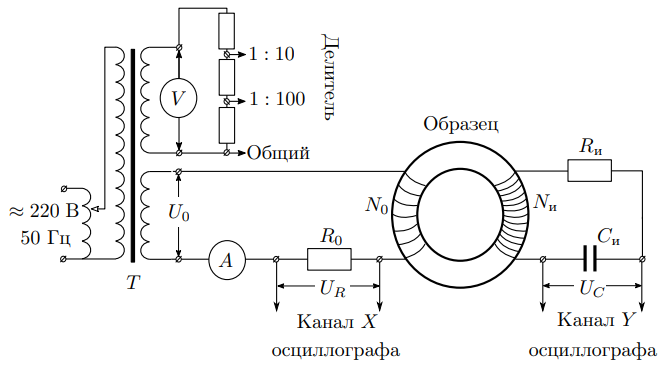
\includegraphics[width = 0.9\textwidth]{Установка.png}
    \caption{ Схема установки для исследования намагничивания образцов}
\end{figure}

\textbf{Обработка данных}:  
\begin{enumerate}
    \item Стутуначала занесём в таблицу параметры каждого из образцов, а также характеристики цепи и интегрирующей ячейки.

\begin{table}[H]\label{tab: Params of material}
    \centering
    \begin{tabular}{|
        >{\columncolor[HTML]{FFFFFF}}c |
        >{\columncolor[HTML]{FFFFFF}}c |
        >{\columncolor[HTML]{FFFFFF}}c |
        >{\columncolor[HTML]{FFFFFF}}c |}
        \hline
        {\color[HTML]{000000} }               & {\color[HTML]{000000} Феррит 1000нн} & {\color[HTML]{000000} Пермаллой 50нп} & {\color[HTML]{000000} Кремнистое железо} \\ \hline
        {\color[HTML]{000000} $N_0$}       & {\color[HTML]{000000} 42}  & {\color[HTML]{000000} 20}   & {\color[HTML]{000000} 25}  \\ \hline
        {\color[HTML]{000000} $N_U$}       & {\color[HTML]{000000} 400} & {\color[HTML]{000000} 300}  & {\color[HTML]{000000} 250} \\ \hline
        {\color[HTML]{000000} $S$, $см^2$} & {\color[HTML]{000000} 3,0} & {\color[HTML]{000000} 0,76} & {\color[HTML]{000000} 2,0} \\ \hline
        {\color[HTML]{000000} $2\pi R$, $см$} & {\color[HTML]{000000} 25,0}          & {\color[HTML]{000000} 13,3}      & {\color[HTML]{000000} 11,0}              \\ \hline
    \end{tabular}
    \caption{Параметры образцов}
\end{table}
\begin{table}[H]\label{tab: Params of system}
    \centering
    \begin{tabular}{|
        >{\columncolor[HTML]{FFFFFF}}c |
        >{\columncolor[HTML]{FFFFFF}}c |}
        \hline
        \cellcolor[HTML]{FFFFFF}{\color[HTML]{000000} $R_0$, Ом} & {\color[HTML]{000000} 0,22} \\ \hline
        {\color[HTML]{000000} $R_и$, кОм}                        & {\color[HTML]{000000} 20}   \\ \hline
        {\color[HTML]{000000} $C_и$, мкФ}                        & {\color[HTML]{000000} 20}   \\ \hline
    \end{tabular}
    \caption{Характеристики цепи и интегрирующей ячейки}
\end{table}
\item После этого получим предельную петлю гистерезиса для каждого из образцов.
\item Далее, рассчитаем коэффициенты преобразования отклонений по осям ЭО в напряженность $H$ и индукцию $B$.
\[H = \frac{I N_0}{2 \pi R} = \frac{K_x N_0}{2 \pi R \cdot R_0},\]
\[B = \frac{R_и C_и K_y}{N_и S}.\]
Результаты занесеём в таблицу ниже.
\begin{table}[H]\label{tab: Scale interval}
    \centering
    \begin{tabular}{|
        >{\columncolor[HTML]{FFFFFF}}c |
        >{\columncolor[HTML]{FFFFFF}}c |
        >{\columncolor[HTML]{FFFFFF}}c |
        >{\columncolor[HTML]{FFFFFF}}c |
        >{\columncolor[HTML]{FFFFFF}}c |}
        \hline
        {\color[HTML]{000000} } &
          {\color[HTML]{000000} $K_x$, мВ} &
          {\color[HTML]{000000} $K_y$, мВ} &
          {\color[HTML]{000000} $H$, А / м} &
          \cellcolor[HTML]{FFFFFF}{\color[HTML]{000000} $B$, Тл / дел} \\ \hline
        {\color[HTML]{000000} Феррит 1000нн} &
          {\color[HTML]{000000} 20} &
          \cellcolor[HTML]{FFFFFF}{\color[HTML]{000000} 10} &
          {\color[HTML]{000000} 15,27} &
          {\color[HTML]{000000} 0,03} \\ \hline
        {\color[HTML]{000000} Пермаллой 50нп} &
          \cellcolor[HTML]{FFFFFF}{\color[HTML]{000000} 10} &
          {\color[HTML]{000000} 10} &
          {\color[HTML]{000000} 6,84} &
          {\color[HTML]{000000} 0,18} \\ \hline
        {\color[HTML]{000000} Кремнистое железо} &
          {\color[HTML]{000000} 50} &
          \cellcolor[HTML]{FFFFFF}{\color[HTML]{000000} 20} &
          {\color[HTML]{000000} 51,65} &
          {\color[HTML]{000000} 0,16} \\ \hline
    \end{tabular}
    \caption{Значения цены деления при различных измерениях}
\end{table}

\item Для каждого образца рассчитаем амплитуду $H_{max}$, соответствующую состоянию насыщения, индукцию насыщения $B_s$, а также коэрцитивную силу $H_c$ и остаточную индукцию $B_r$. Для этого в каждом случае запишем полную ширину и высоту предельной петли ([2$X_s$] и [$2Y_s$]), соответствующие удвоенной амплитуде колебания напряженности $H_s$ и индукции $B_s$ поля в образце в состоянии насыщения, а также двойные амплитуды для коэрцитивного поля [$2X_c$] и остаточной индукции [$2Y_r$]. Погрешность измерений равна половине цены деления осей осциллографа. Полученные результаты запишем в таблицу.
\begin{table}[H]\label{tab: H_s B_s and H_c B_r}
    \centering
    \begin{tabular}{|
        >{\columncolor[HTML]{FFFFFF}}c |
        >{\columncolor[HTML]{FFFFFF}}c 
        >{\columncolor[HTML]{FFFFFF}}c |
        >{\columncolor[HTML]{FFFFFF}}c 
        >{\columncolor[HTML]{FFFFFF}}c |
        >{\columncolor[HTML]{FFFFFF}}c 
        >{\columncolor[HTML]{FFFFFF}}c |}
        \hline
        \cellcolor[HTML]{FFFFFF}{\color[HTML]{000000} } &
          \multicolumn{2}{c|}{\cellcolor[HTML]{FFFFFF}{\color[HTML]{000000} Феррит  1000нн}} &
          \multicolumn{2}{c|}{\cellcolor[HTML]{FFFFFF}{\color[HTML]{000000} Пермаллой 50нп}} &
          \multicolumn{2}{c|}{\cellcolor[HTML]{FFFFFF}{\color[HTML]{000000} \begin{tabular}[c]{@{}c@{}}Кремнистое\\ железо\end{tabular}}} \\ \cline{2-7} 
        \multirow{}{}{\cellcolor[HTML]{FFFFFF}{\color[HTML]{000000} }} &
          \multicolumn{1}{c|}{\cellcolor[HTML]{FFFFFF}{\color[HTML]{000000} Значение}} &
          {\color[HTML]{000000} $\sigma$} &
          \multicolumn{1}{c|}{\cellcolor[HTML]{FFFFFF}{\color[HTML]{000000} Значение}} &
          {\color[HTML]{000000} $\sigma$} &
          \multicolumn{1}{c|}{\cellcolor[HTML]{FFFFFF}{\color[HTML]{000000} Значение}} &
          {\color[HTML]{000000} $\sigma$} \\ \hline
        {\color[HTML]{000000} $H_s$, А / м} &
          \multicolumn{1}{c|}{\cellcolor[HTML]{FFFFFF}{\color[HTML]{000000} 320,727}} &
          {\color[HTML]{000000} 7,636} &
          \multicolumn{1}{c|}{\cellcolor[HTML]{FFFFFF}{\color[HTML]{000000} 85,441}} &
          {\color[HTML]{000000} 3,417} &
          \multicolumn{1}{c|}{\cellcolor[HTML]{FFFFFF}{\color[HTML]{000000} 1239,669}} &
          {\color[HTML]{000000} 25,826} \\ \hline
        {\color[HTML]{000000} $B_s$, Тл} &
          \multicolumn{1}{c|}{\cellcolor[HTML]{FFFFFF}{\color[HTML]{000000} 0,533}} &
          {\color[HTML]{000000} 0,017} &
          \multicolumn{1}{c|}{\cellcolor[HTML]{FFFFFF}{\color[HTML]{000000} 2,895}} &
          {\color[HTML]{000000} 0,088} &
          \multicolumn{1}{c|}{\cellcolor[HTML]{FFFFFF}{\color[HTML]{000000} 1,840}} &
          {\color[HTML]{000000} 0,080} \\ \hline
        {\color[HTML]{000000} $H_c$, А / м} &
          \multicolumn{1}{c|}{\cellcolor[HTML]{FFFFFF}{\color[HTML]{000000} 38,182}} &
          {\color[HTML]{000000} 7,636} &
          \multicolumn{1}{c|}{\cellcolor[HTML]{FFFFFF}{\color[HTML]{000000} 37,594}} &
          \cellcolor[HTML]{FFFFFF}{\color[HTML]{000000} 3,417} &
          \multicolumn{1}{c|}{\cellcolor[HTML]{FFFFFF}{\color[HTML]{000000} 103,306}} &
          \cellcolor[HTML]{FFFFFF}{\color[HTML]{000000} 25,826} \\ \hline
        {\color[HTML]{000000} $B_r$, Тл} &
          \multicolumn{1}{c|}{\cellcolor[HTML]{FFFFFF}{\color[HTML]{000000} 0,233}} &
          {\color[HTML]{000000} 0,017} &
          \multicolumn{1}{c|}{\cellcolor[HTML]{FFFFFF}{\color[HTML]{000000} 2,807}} &
          \cellcolor[HTML]{FFFFFF}{\color[HTML]{000000} 0,088} &
          \multicolumn{1}{c|}{\cellcolor[HTML]{FFFFFF}{\color[HTML]{000000} 0,640}} &
          \cellcolor[HTML]{FFFFFF}{\color[HTML]{000000} 0,080} \\ \hline
    \end{tabular}
    \caption{Вычисленные значения}
\end{table}


\item Теперь постепенно будем уменьшать ток намашничивания от насыщения до нуля и записывать значения полной ширины и высоты петли. Вершины петель лежат на
начальной кривой намагничивания. Результаты измерений приведены в таблице ниже.
\begin{table}[H]\label{tab: Y_s X_s}
    \centering
    \begin{tabular}{|
        >{\columncolor[HTML]{FFFFFF}}c 
        >{\columncolor[HTML]{FFFFFF}}c |
        >{\columncolor[HTML]{FFFFFF}}c 
        >{\columncolor[HTML]{FFFFFF}}c |
        >{\columncolor[HTML]{FFFFFF}}c 
        >{\columncolor[HTML]{FFFFFF}}c |}
        \hline
        \multicolumn{2}{|c|}{\cellcolor[HTML]{FFFFFF}{\color[HTML]{000000} \begin{tabular}[c]{@{}c@{}}Феррит  1000нн\end{tabular}}} &
          \multicolumn{2}{c|}{\cellcolor[HTML]{FFFFFF}{\color[HTML]{000000} \begin{tabular}[c]{@{}c@{}}Пермаллой  50нп\end{tabular}}} &
          \multicolumn{2}{c|}{\cellcolor[HTML]{FFFFFF}{\color[HTML]{000000} \begin{tabular}[c]{@{}c@{}}Кремнистое \\ железо\end{tabular}}} \\ \hline
        \multicolumn{1}{|c|}{\cellcolor[HTML]{FFFFFF}{\color[HTML]{000000} $2X_s$, дел}} &
          {\color[HTML]{000000} $2Y_s$, дел} &
          \multicolumn{1}{c|}{\cellcolor[HTML]{FFFFFF}{\color[HTML]{000000} $2X_s$, дел}} &
          {\color[HTML]{000000} $2Y_s$, дел} &
          \multicolumn{1}{c|}{\cellcolor[HTML]{FFFFFF}{\color[HTML]{000000} $2X_s$, дел}} &
          {\color[HTML]{000000} $2Y_s$, дел} \\ \hline
        \multicolumn{1}{|c|}{\cellcolor[HTML]{FFFFFF}{\color[HTML]{000000} 36}} &
          {\color[HTML]{000000} 30} &
          \multicolumn{1}{c|}{\cellcolor[HTML]{FFFFFF}{\color[HTML]{000000} 16}} &
          {\color[HTML]{000000} 32} &
          \multicolumn{1}{c|}{\cellcolor[HTML]{FFFFFF}{\color[HTML]{000000} 34}} &
          {\color[HTML]{000000} 20} \\ \hline
        \multicolumn{1}{|c|}{\cellcolor[HTML]{FFFFFF}{\color[HTML]{000000} 30}} &
          {\color[HTML]{000000} 30} &
          \multicolumn{1}{c|}{\cellcolor[HTML]{FFFFFF}{\color[HTML]{000000} 12}} &
          {\color[HTML]{000000} 24} &
          \multicolumn{1}{c|}{\cellcolor[HTML]{FFFFFF}{\color[HTML]{000000} 26}} &
          {\color[HTML]{000000} 18} \\ \hline
        \multicolumn{1}{|c|}{\cellcolor[HTML]{FFFFFF}{\color[HTML]{000000} 24}} &
          {\color[HTML]{000000} 27} &
          \multicolumn{1}{c|}{\cellcolor[HTML]{FFFFFF}{\color[HTML]{000000} 11}} &
          {\color[HTML]{000000} 17} &
          \multicolumn{1}{c|}{\cellcolor[HTML]{FFFFFF}{\color[HTML]{000000} 20}} &
          {\color[HTML]{000000} 16} \\ \hline
        \multicolumn{1}{|c|}{\cellcolor[HTML]{FFFFFF}{\color[HTML]{000000} 20}} &
          {\color[HTML]{000000} 25} &
          \multicolumn{1}{c|}{\cellcolor[HTML]{FFFFFF}{\color[HTML]{000000} 10}} &
          {\color[HTML]{000000} 12} &
          \multicolumn{1}{c|}{\cellcolor[HTML]{FFFFFF}{\color[HTML]{000000} 15}} &
          {\color[HTML]{000000} 15} \\ \hline
        \multicolumn{1}{|c|}{\cellcolor[HTML]{FFFFFF}{\color[HTML]{000000} 18}} &
          {\color[HTML]{000000} 23} &
          \multicolumn{1}{c|}{\cellcolor[HTML]{FFFFFF}{\color[HTML]{000000} 9}} &
          {\color[HTML]{000000} 8} &
          \multicolumn{1}{c|}{\cellcolor[HTML]{FFFFFF}{\color[HTML]{000000} 10}} &
          {\color[HTML]{000000} 12} \\ \hline
        \multicolumn{1}{|c|}{\cellcolor[HTML]{FFFFFF}{\color[HTML]{000000} 15}} &
          {\color[HTML]{000000} 20} &
          \multicolumn{1}{c|}{\cellcolor[HTML]{FFFFFF}{\color[HTML]{000000} 8}} &
          {\color[HTML]{000000} 6} &
          \multicolumn{1}{c|}{\cellcolor[HTML]{FFFFFF}{\color[HTML]{000000} 7}} &
          {\color[HTML]{000000} 9} \\ \hline
        \multicolumn{1}{|c|}{\cellcolor[HTML]{FFFFFF}{\color[HTML]{000000} 13}} &
          {\color[HTML]{000000} 18} &
          \multicolumn{1}{c|}{\cellcolor[HTML]{FFFFFF}{\color[HTML]{000000} 8}} &
          {\color[HTML]{000000} 4} &
          \multicolumn{1}{c|}{\cellcolor[HTML]{FFFFFF}{\color[HTML]{000000} 4}} &
          {\color[HTML]{000000} 6} \\ \hline
        \multicolumn{1}{|c|}{\cellcolor[HTML]{FFFFFF}{\color[HTML]{000000} 10}} &
          {\color[HTML]{000000} 15} &
          \multicolumn{1}{c|}{\cellcolor[HTML]{FFFFFF}{\color[HTML]{000000} }} &
          {\color[HTML]{000000} } &
          \multicolumn{1}{c|}{\cellcolor[HTML]{FFFFFF}{\color[HTML]{000000} 3}} &
          {\color[HTML]{000000} 5} \\ \hline
        \multicolumn{1}{|c|}{\cellcolor[HTML]{FFFFFF}{\color[HTML]{000000} 8}} &
          {\color[HTML]{000000} 11} &
          \multicolumn{1}{c|}{\cellcolor[HTML]{FFFFFF}{\color[HTML]{000000} }} &
          {\color[HTML]{000000} } &
          \multicolumn{1}{c|}{\cellcolor[HTML]{FFFFFF}{\color[HTML]{000000} }} &
          {\color[HTML]{000000} } \\ \hline
    \end{tabular}
    \caption{Результаты измерений}
\end{table}

\item По данным из таблицы оценим начальное и максимальное значения дифференциальной магнитной проницаемости $\mu_{диф}$. Результаты занесём в таблицу.
\begin{table}[H]\label{tab: mu nach and mu max}
    \centering
    \begin{tabular}{|
        >{\columncolor[HTML]{FFFFFF}}c |
        >{\columncolor[HTML]{FFFFFF}}c |
        >{\columncolor[HTML]{FFFFFF}}c |
        >{\columncolor[HTML]{FFFFFF}}c |}
        \hline
        {\color[HTML]{000000} } &
          {\color[HTML]{000000} Феррит  1000нн} &
          {\color[HTML]{000000} Пермаллой  50нп} &
          {\color[HTML]{000000} \begin{tabular}[c]{@{}c@{}}Кремнистое\\ железо\end{tabular}} \\ \hline
        {\color[HTML]{000000} $\mu_{нач}$, $10^3$} &
          {\color[HTML]{000000} 3,127} &
          {\color[HTML]{000000} 41,883} &
          {\color[HTML]{000000} 24,651} \\ \hline
        \cellcolor[HTML]{FFFFFF}{\color[HTML]{000000} $\mu_{макс}$, $10^3$} &
          {\color[HTML]{000000} 3,127} &
          {\color[HTML]{000000} 146,590} &
          \cellcolor[HTML]{FFFFFF}{\color[HTML]{000000} 24,651} \\ \hline
    \end{tabular}
    \caption{Значения максимальной и начальной магнитной проницаемости }
\end{table}

\item Измерим постоянную $RC$-цепочки $\tau_и$, для этого, при условии $U_{вых} \ll U_{вх}$, получаем формулу
\[\frac{U_{вых}}{U_{вх}} \approx \frac{1}{\omega_0 \tau},\]
отсюда, измеряя входное напряжение и напряжение на конденсаторе, найдём постоянную $\tau_и$. Для этого при одном и том же значении тока будем измерять количество делений, занимаемых линией сигнала, на осциллографе. Результат приведён в таблице ниже.
\begin{table}[H]\label{tab: RC const}
    \centering
    \begin{tabular}{|
        >{\columncolor[HTML]{FFFFFF}}c |
        >{\columncolor[HTML]{FFFFFF}}c |
        >{\columncolor[HTML]{FFFFFF}}c |}
        \hline
        {\color[HTML]{000000} }          & {\color[HTML]{000000} $K_y$, мВ} & {\color[HTML]{000000} $2y$, дел.} \\ \hline
        {\color[HTML]{000000} $U_{вх}$}  & {\color[HTML]{000000} 1000}      & {\color[HTML]{000000} $31 \pm 0,5$}         \\ \hline
        {\color[HTML]{000000} $U_{вых}$} & {\color[HTML]{000000} 10}        & {\color[HTML]{000000} $28 \pm 0,5$}         \\ \hline
    \end{tabular}
    \caption{Данные для вычисления постоянной $RC$-цепи}
\end{table}
\[\tau_и = \frac{U_{вх}}{U_{вых}} \frac{1}{\omega_0} = (352 \pm 8) \cdot 10^{-3} \text{ с},\]
\[R_и \cdot C_и = 0,4 \text{ с}.\]
Как видим, значение отличается от теоретического на $\varepsilon \approx 12 \%$. 

Далее, проверим справедливость предположения $U_{вых} \ll U_{вх}$, которое выполняется, если $R_и \gg \frac{1}{\omega_0 C_и}$.
\[\frac{1}{\omega_0 C_и} \approx 159,15 \text{ Ом} \ll R = 20000 \text{ Ом}.\]
Таким образом, соотношение выполняется, и поэтому можно использовать упрощенную формулу для нахождения индукции магнитного поля внутри образца. 

\item Последним пунктом сведём результаты работы в таблицу, сравним полученные значения с табличными. 
\begin{table}[H]\label{tab: final tab}
    \centering
    \begin{tabular}{|
        >{\columncolor[HTML]{FFFFFF}}c |
        >{\columncolor[HTML]{FFFFFF}}c 
        >{\columncolor[HTML]{FFFFFF}}c |
        >{\columncolor[HTML]{FFFFFF}}c 
        >{\columncolor[HTML]{FFFFFF}}c |
        >{\columncolor[HTML]{FFFFFF}}c 
        >{\columncolor[HTML]{FFFFFF}}c |}
        \hline
        {\color[HTML]{000000} } &
          \multicolumn{2}{c|}{\cellcolor[HTML]{FFFFFF}{\color[HTML]{000000} Феррит  1000нн}} &
          \multicolumn{2}{c|}{\cellcolor[HTML]{FFFFFF}{\color[HTML]{000000} Пермаллой 50нп}} &
          \multicolumn{2}{c|}{\cellcolor[HTML]{FFFFFF}{\color[HTML]{000000} \begin{tabular}[c]{@{}c@{}}Кремнистое\\ железо\end{tabular}}} \\ \hline
        {\color[HTML]{000000} } &
          \multicolumn{1}{c|}{\cellcolor[HTML]{FFFFFF}{\color[HTML]{000000} эксп.}} &
          {\color[HTML]{000000} справ.} &
          \multicolumn{1}{c|}{\cellcolor[HTML]{FFFFFF}{\color[HTML]{000000} эксп.}} &
          {\color[HTML]{000000} справ.} &
          \multicolumn{1}{c|}{\cellcolor[HTML]{FFFFFF}{\color[HTML]{000000} эксп.}} &
          {\color[HTML]{000000} справ.} \\ \hline
        {\color[HTML]{000000} $H_c$, А / м} &
          \multicolumn{1}{c|}{\cellcolor[HTML]{FFFFFF}{\color[HTML]{000000} $38,182 \pm 7,636$}} &
          {\color[HTML]{000000} 20,000} &
          \multicolumn{1}{c|}{\cellcolor[HTML]{FFFFFF}{\color[HTML]{000000} $37,594 \pm 3,417$}} &
          {\color[HTML]{000000} 18,000} &
          \multicolumn{1}{c|}{\cellcolor[HTML]{FFFFFF}{\color[HTML]{000000} $103,306 \pm 25,826$}} &
          {\color[HTML]{000000} 8,000} \\ \hline
        {\color[HTML]{000000} $B_s$, Тл} &
          \multicolumn{1}{c|}{\cellcolor[HTML]{FFFFFF}{\color[HTML]{000000} $0,533 \pm 0,017$}} &
          {\color[HTML]{000000} 7,636} &
          \multicolumn{1}{c|}{\cellcolor[HTML]{FFFFFF}{\color[HTML]{000000} $2,895 \pm 0,088$}} &
          {\color[HTML]{000000} 1,500} &
          \multicolumn{1}{c|}{\cellcolor[HTML]{FFFFFF}{\color[HTML]{000000} $1,840 \pm 0,080$}} &
          {\color[HTML]{000000} 2,000} \\ \hline
        {\color[HTML]{000000} $\mu_{нач}$, $10^3$} &
          \multicolumn{1}{c|}{\cellcolor[HTML]{FFFFFF}{\color[HTML]{000000} 3,127}} &
          {\color[HTML]{000000} 1,000} &
          \multicolumn{1}{c|}{\cellcolor[HTML]{FFFFFF}{\color[HTML]{000000} 41,883}} &
          {\color[HTML]{000000} 7 - 40} &
          \multicolumn{1}{c|}{\cellcolor[HTML]{FFFFFF}{\color[HTML]{000000} 24,651}} &
          {\color[HTML]{000000} 1,500} \\ \hline
        {\color[HTML]{000000} $\mu_{max}$, $10^3$} &
          \multicolumn{1}{c|}{\cellcolor[HTML]{FFFFFF}{\color[HTML]{000000} 3,127}} &
          {\color[HTML]{000000} 3,000} &
          \multicolumn{1}{c|}{\cellcolor[HTML]{FFFFFF}{\color[HTML]{000000} 146,590}} &
          {\color[HTML]{000000} 40 - 1200} &
          \multicolumn{1}{c|}{\cellcolor[HTML]{FFFFFF}{\color[HTML]{000000} 24,651}} &
          {\color[HTML]{000000} 40,000} \\ \hline
    \end{tabular}
    \caption{Результаты работы}
\end{table}

\end{enumerate}

\textbf{Вывод}: В данной работе были исследованы ферромагнитные свойства феррита 1000нн, пермаллоя 50нп и кремнистого железа. Для каждого изх образцов была получена предельная петля гистерезиса После этого для каждого материала были рассчитаны: коэрцитивная сила $H_c$, индукция насыщения $B_s$, начальная магнитная проницаемость $\mu_{нач}$ и максимальная магнитная проницаемость $\mu_{max}$, значения были сравнены со справочными, результаты приведены в таблице выше. Также, была измерена постоянная $RC$-цепочки $\tau_и$, после чего была проверена справедливость приближений, использовавшихся в работе. 

%%%%%%%%%%%%%%%%%%%%%%%%% Графики
\newpage
\begin{figure}[H]\label{fig: Ferrit  pred petlya}
    \centering
    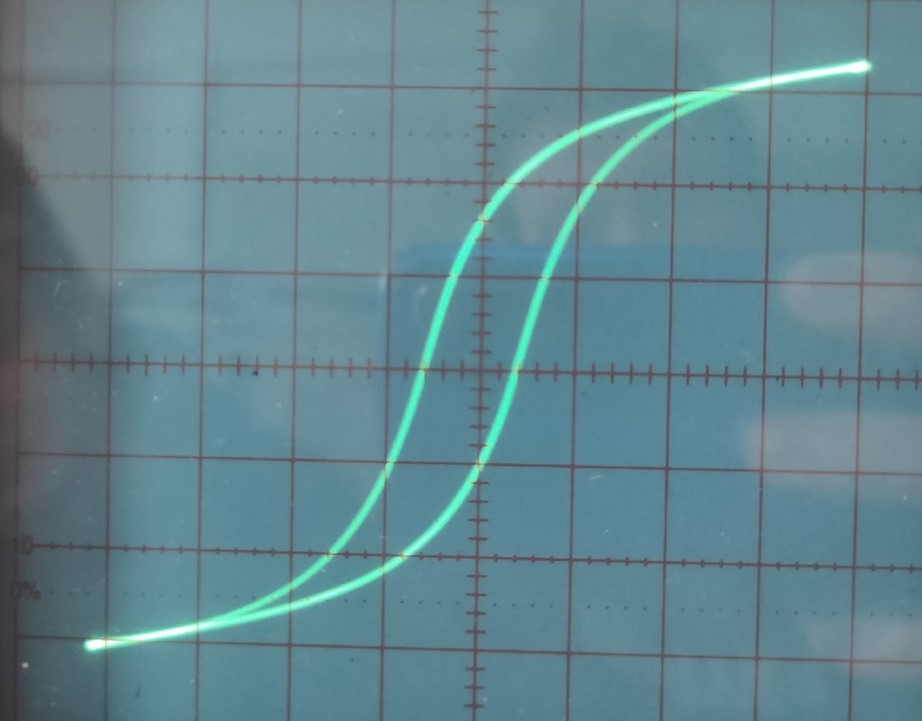
\includegraphics[width = \textwidth]{гистерезис Феррит.png}
    \caption{Предельная петля гистерезиса феррита 1000нн}
\end{figure}

%%%%%%%%%%%%%%%%%%%%%%%%%
\end{document}
